\documentclass[a4paper,12pt,headings=small,ngerman,bibliography=totoc]{scrartcl}
\usepackage[ngerman]{babel}
\usepackage[utf8]{inputenc}
\usepackage[headsepline]{scrlayer-scrpage}

\usepackage{amssymb,graphicx}
\clearscrheadings
\pagestyle{scrheadings}
\usepackage[left=2.5cm,right=2.5cm,top=3cm,bottom=2.5cm]{geometry}
\usepackage[onehalfspacing]{setspace}
\usepackage{microtype}
\ofoot{\pagemark}
\footskip1cm
\setkomafont{sectioning}{\normalfont\normalcolor\bfseries}
\usepackage[osf,sc]{mathpazo}
\usepackage{url}
\clubpenalty = 10000
\widowpenalty = 10000 \displaywidowpenalty = 10000

\usepackage[usenames,
	    dvipsnames,
	    svgnames]{xcolor}

\usepackage[babel,german=quotes]{csquotes}
\usepackage{url}
\usepackage{soul}

%%% Für Bildunterschriften %%%
\usepackage{caption}

%%% Für Bilder im Text %%%
\usepackage{wrapfig}

%%% Für Mathe %%%
\usepackage[fleqn]{amsmath}
\usepackage{commath}
\usepackage{amstext}
\allowdisplaybreaks
%%% Für schräge Bruchstriche %%%
\usepackage{nicefrac}
%%% Rechtecke %%%
\usepackage{amsfonts}

%%% Für Textübergreifende Numerierung %%%
\usepackage{enumitem}
\renewcommand{\labelenumi}{\alph{enumi})}

%%% Für Abkürzungen %%%
\usepackage{acronym}

%%% Fuer Querformat fuer einzelne Seiten %%%
\usepackage{lscape}

%%%% Überschriften bis subsubsubsection (paragraph) %%%
\setcounter{secnumdepth}{5}

\setkomafont{dictumtext}{\itshape\small}
\setkomafont{dictumauthor}{\small}
\renewcommand*\dictumwidth{\linewidth}
\renewcommand*\dictumauthorformat[1]{--- #1}
\renewcommand*\dictumrule{}

%%% Für Quotes %%%
\usepackage[ngerman]{varioref}
\usepackage{hyperref}
 \hypersetup{%draft, 								% no hyperlinking at all (useful in b/w printouts)
    colorlinks=true, breaklinks=true,
    urlcolor=Black, linkcolor=Black, citecolor=Black,
    linktoc=page, %
    bookmarksnumbered, bookmarksopenlevel=1, bookmarksdepth = section,%
    pdfstartview=FitV,
    }
\setlength{\parindent}{0em}
\usepackage{cleveref}
\crefname{paragraph}{Abschnitt}{Abschnitt}

\usepackage[bibencoding=utf8,
			sortlocale=de,
			style=authoryear-icomp,
			pagetracker=true,
			autocite=inline,
			backrefstyle=three+,
			date=short,
			sorting=nty,
			backend=biber]{biblatex}
			
\bibliography{Literaturverzeichnis}

%%% urldate in eckigen Klammern %%%
\DeclareFieldFormat{urldate}{\mkbibbrackets{#1}}
%%% URL: = Verfügbar unter: %%%
\DeclareFieldFormat{url}{{Verfügbar unter:}\space\url{#1}}
%%% Abstand zwischen den Literaturangaben %%%
\setlength{\bibitemsep}{1.3em}
%%% statt und ein & %%%
\renewcommand*{\finalnamedelim}{\space\&\space}
%%% Nachname, Vorname, immer %%%
\DeclareNameAlias{sortname}{last-first}

%%% Kopfzeile %%%
\automark[section]{section}
\renewcommand*{\headfont}{\normalfont}
\setkomafont{pageheadfoot}{}
\renewcommand*{\sectionmarkformat}{} 

%%% Damit das Abbildungsverzeichnis im Inhaltsverzeichnis abgebildet wird %%%
\usepackage{tocbibind}
\renewcommand{\listoffigures}{\begingroup
  \tocchapter
  \tocfile{\listfigurename}{lof}
  \endgroup}
  
%%% Für SI Einheiten %%%
\usepackage[binary-units]{siunitx}
\sisetup{
  locale = DE ,
  detect-all
}

%Für Tabellen
\usepackage{array}
% Für Seitenübergreifende Tabellen
\usepackage{longtable}
% Für Tabellen mit vertikal und horizontal zentriertem Inhalt
\newcolumntype{B}[1]{>{\centering\arraybackslash}m{#1}}

\begin{document}

\pagenumbering{gobble}
\pagestyle{empty}


\begin{center}
  \Large{Berufliches Schulzentrum für Elektrotechnik Dresden}\\
\end{center}

\begin{center}
  \Large{Fachbereich Informationstechnik}
\end{center}
\begin{verbatim}

\end{verbatim}
\begin{center}
  \textbf{\LARGE{Pflichtenheft}}
\end{center}

\begin{center}
  \Large{Lernfeld 9 - Projekt 3}
\end{center}

\vspace{\fill}

\begin{flushleft}
  \begin{tabular}{lll}
                            &                                                & \\
                            &                                                & \\
                            &                                                & \\
                            &                                                & \\
                            &                                                & \\
                            &                                                & \\
    \textbf{Auftraggeber:}  & Doubtful-Joy SE                                & \\
    \textbf{Auftragnehmer:} & High-Secure GmbH - Projektteam IT20/2 Gruppe 7 & \\
    \textbf{Auftragsdatum:} & 2021.11.15                                     & \\
                            &                                                & \\
    \textbf{Historie:}      &                                                & \\
  \end{tabular}
\end{flushleft}

\newpage
%%% Inhaltsverzeichnis einfügen %%%
\tableofcontents
\cleardoublepage

\newpage
\pagestyle{scrheadings}
\pagenumbering{arabic}
\ohead{Projekt 3, Lehrjahr 21/22}
\ihead{\rightmark}

%%% Was muss in ein Pflichtenheft: https://www.vario-software.de/lexikon/pflichtenheft/

\section{Auftraggeber und Auftragnehmer }

Beim Auftraggeber handelt es sich um die Gaming-Plattform \textbf{Doubtful-Joy SE}. Ansprechpartner sind

\begin{table}[htbp]
  \centering
  \renewcommand{\arraystretch}{1.25}
  \caption{Ansprechpartner Auftraggeber}
  \begin{tabular}{lllll}
    Funktion     & Name   & Vorname & Email                                 \\
    \hline
    Auftraggeber & Hempel & Steffen & \flq{}hempel@bszetdd.lernsax.de\frq{} \\
  \end{tabular}
  \label{tab:Auftraggeber}
\end{table}

Beim Auftragnehmer handelt es sich um das \textbf{High-Secure GmbH - Projektteam IT20/2 Gruppe 7}. Ansprechpartner sind

\begin{table}[htbp]
  \centering
  \renewcommand{\arraystretch}{1.25}
  \caption{Ansprechpartner Auftragnehmer}
  \begin{tabular}{lllll}
    Funktion          & Name      & Vorname  & Email                                         \\ \hline
    Projektmanager    & Egermann  & Péter    & \flq{}i20egermannpe@bszetdd.lernsax.de\frq{}  \\
    Teamleiter        & Leyrer    & Johannes & \flq{}i20leyrerjo@bszetdd.lernsax.de\frq{}    \\
    Netzwerkingenieur & Brethfeld & Vinzenz  & \flq{}i20brethfeldvi@bszetdd.lernsax.de\frq{} \\
  \end{tabular}
  \label{tab:Auftragnehmer}
\end{table}


\section{Ausgangslage}

Die existierende Support-Infrastruktur der Gaming-Plattform Doubtful-Joy SE lässt sich über Mail und Telefon kontaktieren. Dabei wird jeder Anruf und jede Mail individuell von einem Mitarbeiter als Ticket gespeichert und in einem zentralen Laufwerk abgelegt. Effizienz, Ordnung und Übersichtlichkeit sind nicht ausreichend vorhanden.


\section{Projektziel}

Die Gaming-Plattform Doubtful-Joy SE möchte ihre existierende Support-Infrastruktur durch ein Ticketsystem ersetzen. Dieses soll für Kunden und Mitarbeiter über ein Web-Interface erreichbar sein. Tickets sollen über dieses direkt erstellt und mit beliebig vielen Attachments versehen werden können.

Außerdem soll eine Segmentierung der Netzinfrastruktur mit einer sichereren Trennung von öffentlich erreichbaren Diensten und dem Intranet eingerichtet werden. Ebenso sollen die internen Dienste DNS und DHCP auf einem separatem System bereitgestellt werden, um eine Abhängigkeit von der Firewall auszuschließen.

Doubtful-Joy SE setzt auf RedHat und binärkompatible Systeme, weshalb diese System-Strategie weiterhin umgesetzt werden soll.


\section{Funktionsspezifikation}

Von der Realisierung sind betroffen:

\begin{description}
  \item[Manware] \
    \begin{itemize}
      \item Projektteam IT20/2 Gruppe 7
      \item Support-Mitarbeiter des Auftraggeber
      \item IT-Mitarbeiter des Autraggebers
    \end{itemize}
  \item[Orgware] \
    \begin{itemize}
      \item Sicherheitsanforderungen
      \item Benutzerhandbuch
      \item Benutzerschulung
    \end{itemize}
  \item[Hardware] \
    \begin{itemize}
      \item Server
      \item Mitarbeiter-PCs
    \end{itemize}
  \item[Software] \
    \begin{itemize}
      \item VM-Ware
      \item Datenbank-Server
      \item Web-Server
      \item Firewall-System
      \item DNS
      \item DHCP
    \end{itemize}
\end{description}


\section{Datenspezifikation}

Da von etwa 1000 Telefonanrufen  und Emails pro Tag ausgegangen wird, kann dies etwa 1:1 in 1000 Tickets übertragen werden. Der Speicherbedarf pro Ticket wird hier im Schnitt auf etwa \SI{5}{\mega\byte} geschätzt, da wahrscheinlich häufiger Anhänge in Bildform zur besseren Problembeschreibung genutzt werden. Zusätzlich wird davon ausgegangen, dass die Daten zur Sicherheit und Nachvollziehbarkeit für ein Jahr gespeichert werden, wodurch die Datenbank \SI{1830}{\giga\byte} Speicher in einem Jahr benötigt.

\begin{align*}
  \frac{\SI{5}{\mega\byte}}{\text{Ticket}} \cdot \frac{1000\text{ Ticket}}{\text{Tag}} & = \frac{\SI{5000}{\mega\byte}}{\text{Tag}}                                                                  \\
  \frac{\SI{5000}{\mega\byte}}{\text{Tag}} \cdot 365 \text{Tage}                       & = \frac{\SI{1825000}{\mega\byte}}{\text{Jahr}} \stackrel{\wedge}= \frac{\SI{1830}{\giga\byte}}{\text{Jahr}}
\end{align*}


Da es keine Good-Practice ist, die Bilder in der Datenbank zu speichern, wird nur der Dateipfad zu den Bildern in der Datenbank hinterlegt, die Bilder selbst liegen auf der Festplatte des Webservers. Damit verringert sich der geschätzte Speicherbedarf der Datenbank auf etwa \SI{183}{\giga\byte} pro jahr.

\begin{align*}
  \frac{\SI{0.5}{\mega\byte}}{\text{Ticket}} \cdot \frac{\text{Ticket}}{\text{Tag}} = \frac{\SI{500}{\mega\byte}}{\text{Tag}} \stackrel{\wedge}= \frac{\SI{183}{\giga\byte}}{\text{Jahr}}
\end{align*}

Die Bilder selbst benötigen zum aktuellen Stand auf der Festplatte \SI{1643}{\giga\byte} Speicher pro Jahr.

\begin{align*}
  \frac{\SI{4.5}{\mega\byte}}{\text{Bild}} \cdot 1000 \frac{\text{Bild}}{\text{Tag}} = \frac{\SI{4500}{\mega\byte}}{\text{Tag}} \stackrel{\wedge}= \frac{\SI{1643}{\giga\byte}}{\text{Jahr}}
\end{align*}

Die Art von Daten sind personenbezogene Daten in Text- und Bildform.

Der Datenfluss geht vom Clienten zur DMZ und zur Bearbeitung dann zum PC des Support-Mitarbeiters, grafisch dargestellt in \vref{fig:Schnittstellenspezifikation}.


\newpage
\section{Schnittstellenspezifikation}

\begin{figure}[htbp]
  \centering
  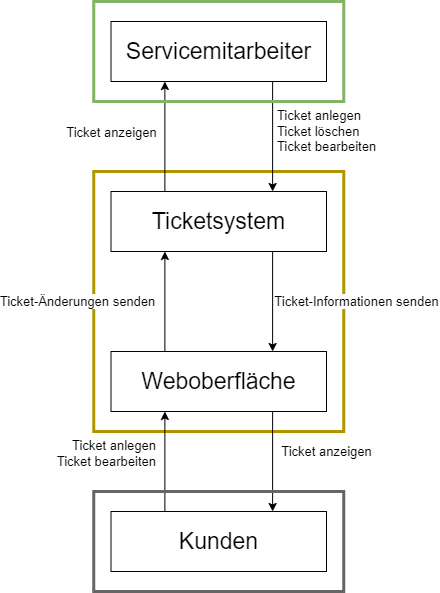
\includegraphics[width=0.75\textwidth]{data/Schnittstellendiagramm.png}
  \caption{Schnittstellenspezifikation}
  \label{fig:Schnittstellenspezifikation}
\end{figure}


\section{Rahmenbedigungen}

Der Auftraggeber hat folgende Ressourcen bereitzustellen und Mitwirklungspflichten:

\begin{itemize}
  \item Server
  \item Mitarbeiter-PCs
  \item Zugriff auf alle zu bearbeitenden Systeme und Zutritt zu den notwendigen Räumlichkeiten
  \item Kooperation und eventuell notwendigen lokalen Support
\end{itemize}


\section{Qualitätsbetrachtung}

Die Arbeitspakete werden stets wahrend der Erstellung nach der Fertigstellung auf Funktion und Qualität überprüft.

Wöchentlich werden Meetings abgehalten um den Stand des Projekts zu erörtern und auf eventuell auftretende Probleme zeitnah reagieren zu können.

Die Zeitplanung und damit der Aufwand ist in \vref{fig:Gantt} in kleinem Format und groß in \vref{app:Gantt} zu sehen.  Für einen langfristigen Support für nach der der Fertigstellung wird ein zusätzliches Angebot vorgelegt.


\section{Projektplanung}

Die Projektplanung ist im Projektstrukturplan, zu sehen in \vref{fig:Projektstrukturplan}, und im Gantt-Diagramm, zu sehen in \vref{fig:Gantt}, bzw. \vref{app:Gantt}, abgebildet.
Ebenso wird der im Anhang \cpageref{app:Netzwerkplan} zu betrachtende Netzwerkplan \vref{app:Netzwerkplan} umgesetzt.

\begin{figure}[htbp]
  \centering
  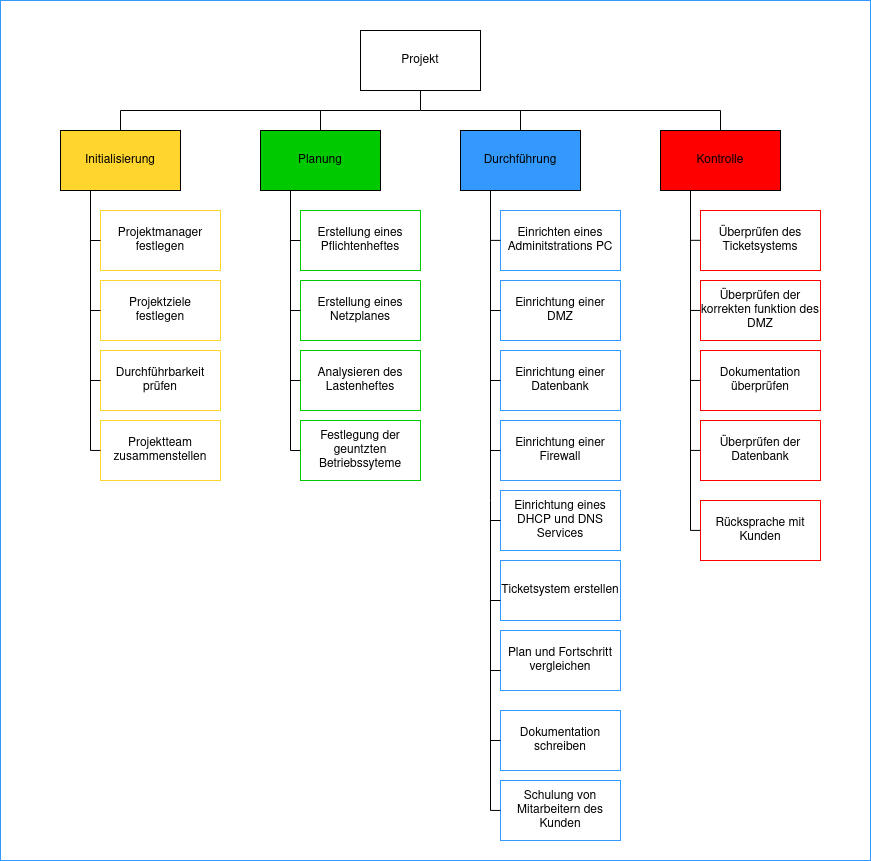
\includegraphics[width=0.75\textwidth]{data/Projektstrukturplan.png}
  \caption{Projektstrukturplan}
  \label{fig:Projektstrukturplan}
\end{figure}

\begin{figure}[htbp]
  \centering
  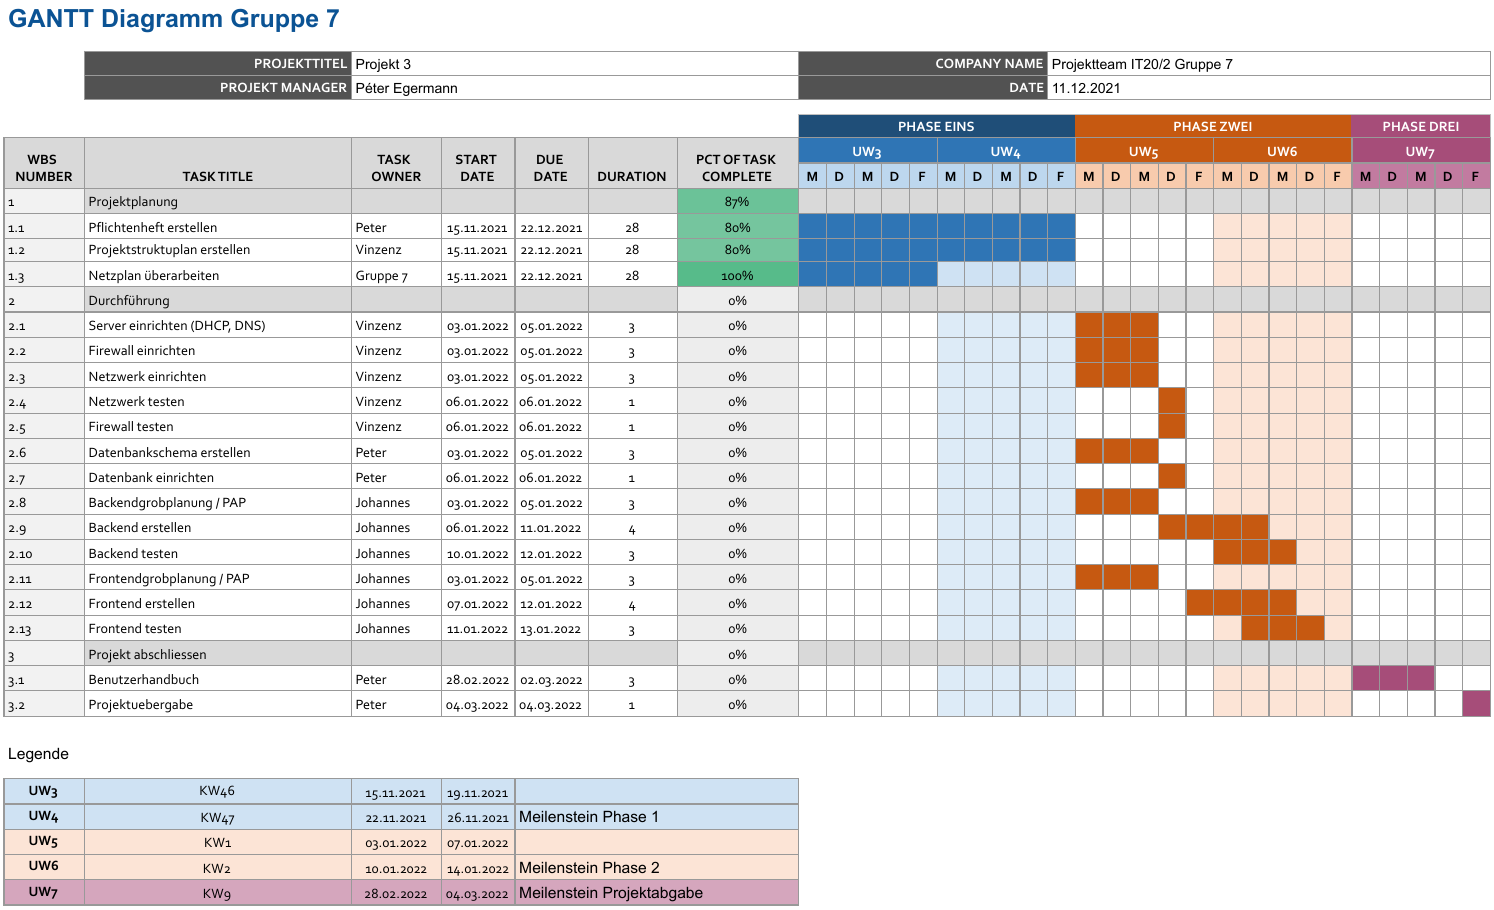
\includegraphics[width=0.95\textwidth]{data/Gantt.png}
  \caption{Gantt-Diagramm}
  \label{fig:Gantt}
\end{figure}


\section{Kosten-Nutzen-Analyse}

Eine Kosten-Nutzen-Analyse ist zum jetzigen Zeitpunkt nicht notwendig, da der Support erst mal entlastet werden muss. Dies ist durch das neue System auf jeden Fall der Fall, da quasi der Kunde das Ticket erstellt und nicht der Support-Mitarbeiter. Somit kann sich voll auf das Beheben des Problems konzentriert werden.


\newpage

\appendix
\ihead{Anhang}


\section{Gantt-Diagramm}

\begin{figure}[h!]
  \centering
  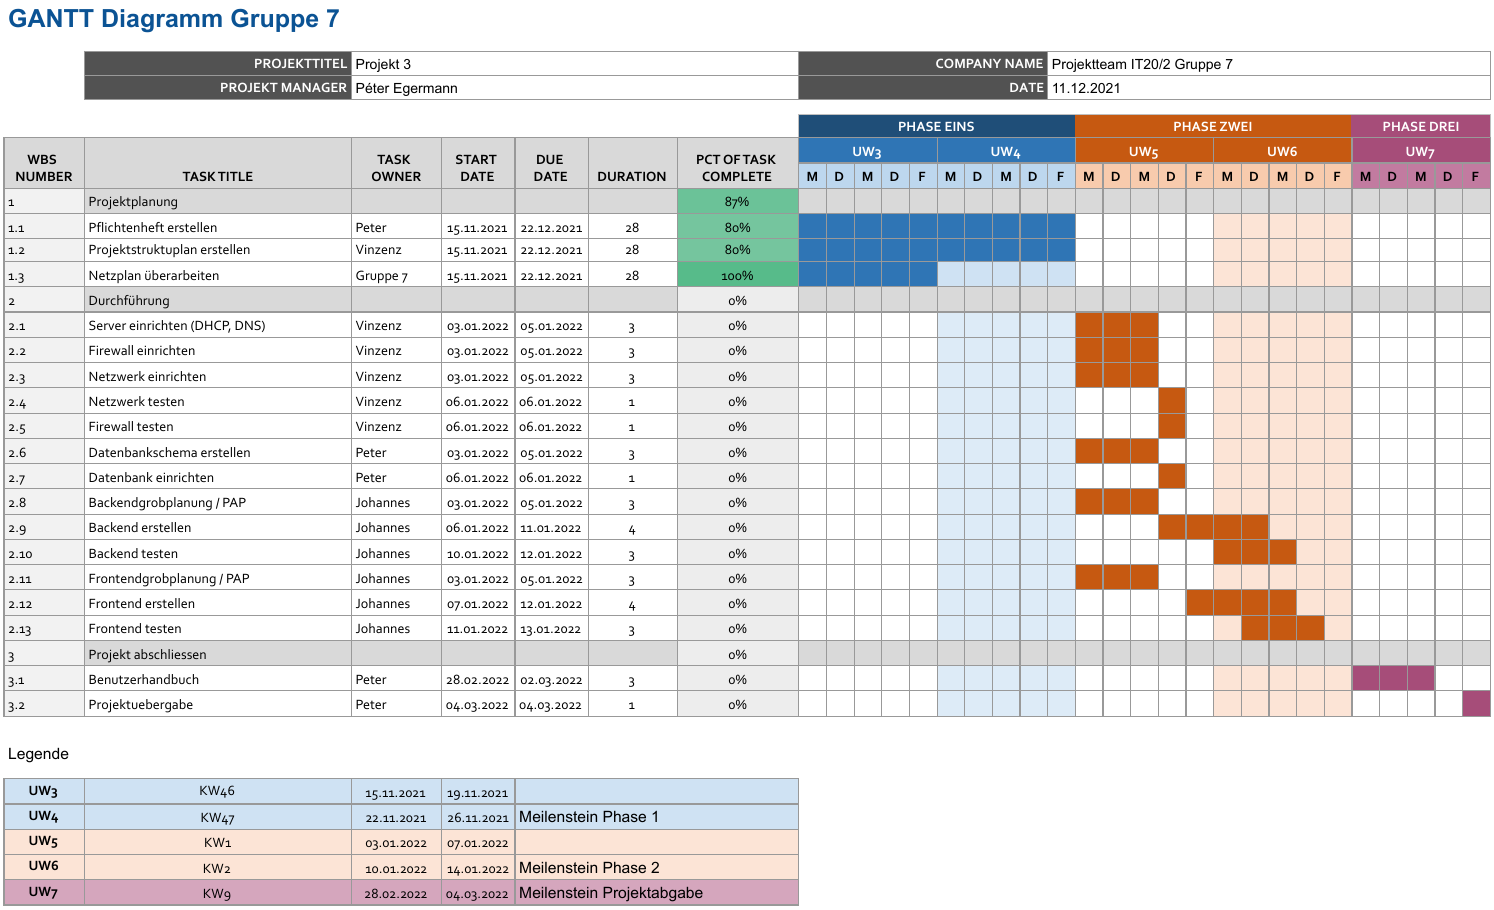
\includegraphics[angle=90,origin=c,width=0.8\textwidth]{data/Gantt.png}
  \caption{Gantt-Diagramm}
  \label{app:Gantt}
\end{figure}


\section{Netzwerkplan}

\begin{figure}[h!]
  \centering
  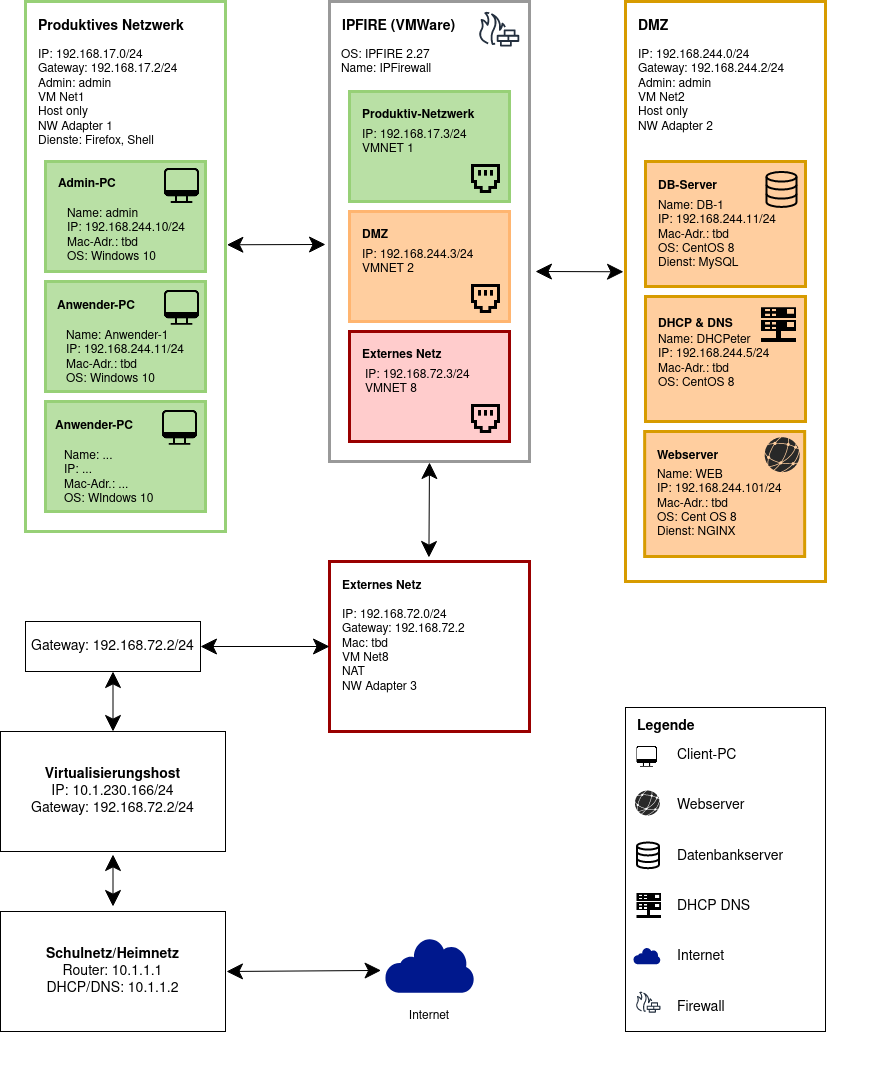
\includegraphics[width=0.95\textwidth]{data/Netzwerkplan.png}
  \caption{Netzwerkplan}
  \label{app:Netzwerkplan}
\end{figure}

\end{document}
